
\subsection{Klassen und ihre Funktionen}

\begin{figure}[h]
	\begin{minipage}{\textwidth}
		\centering
		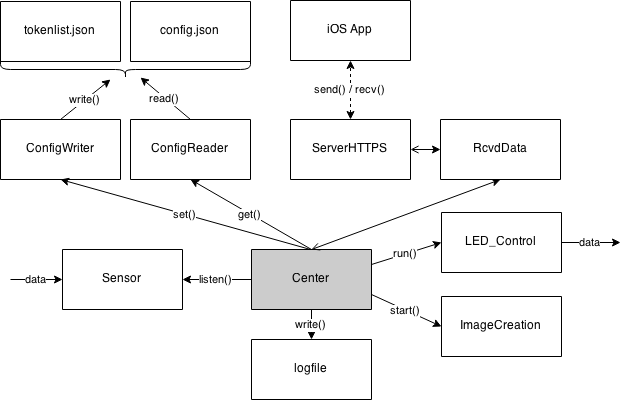
\includegraphics[width=\textwidth]{./data/ApplicationConcept.png}
		\caption{Anwendungsstruktur Server-Anwendung}
	\end{minipage}
\end{figure}

\begin{itemize}
\item Center\\
Die Klasse 'Center' stellt die zentrale Stelle in der Anwendung dar, an der alle Informationen zusammen laufen und verwaltet werden.
\item ServerHTTPS\\
Hier läuft der Webserver, welcher Nachrichten empfängt und sendet. Empfangene Nachrichten werden an die Klasse 'RcvdData' übergeben.
\item RcvdData\\
Hier werden die empfangenen Nachrichten ausgewertet und entsprechende Antworten generiert. Diese werden an den Webserver zurück gegeben und abgesendet. Die Prüfung der Korrektheit der einzelnen Protokollbestandteile findet ebenfalls hier statt. Wenn alle Überprüfungen erfolgreich sind, werden die Befehle an 'Center' weiter gegeben und dort ausgeführt.
\item Sensor\\
In der Klasse 'Sensor' werden die einzelnen Bewegungssensoren überwacht. Falls eine Bewegung detektiert wird, so werden in 'Center' die notwendigen Methoden aufgerufen um die LEDs an- oder auszuschalten.
\item LED-Control\\
Die Klasse 'LED\_Control' verwaltet die eingerichteten LEDs und steuert diese. Hier werden auch die möglichen Effekte gesteuert. Die Methoden in dieser Klasse werden aus der Klasse 'Center' aufgerufen. Ein Zugriff in die andere Richtung ist nicht möglich.
\item ConfigReader / ConfigWriter\
Diese beiden Klassen bieten die Möglichkeit die Konfigurationsdatei config.json zu lesen und zu schreiben. In der Konfiguration werden Informationen wie Anzahl der LEDs, Passworthash oder Adresse der Netzwerkkamera abgespeichert. Die Konfigurationsdatei wird beim Installationsvorgang erstellt.
\item ImageCreation\\
Abrufen von Bildmaterial von der Netzwerkkamera oder vom Server findet ausschließlich über die Klasse 'ImageCreation' statt. Die Klasse ruft die Informationen ab und filtert das Bildmaterial. Außerdem ist sie fähig, die gespeicherten Bilder zu Verwalten und das FTP-Verzeichnis zu mounten.
\item Logfile\\
Im Logfile werden unter anderem auftretende Fehler gespeichert.
\end{itemize}

\subsection{Auswertung empfangener Daten}
Da die Daten anhand des ausgearbeiteten Protokolls übertragen werden, können sie als String sehr einfach an den ':' aufgesplittet werden. Im Anschluss werden sie einzelnen Variablen zugewissen (bessere Lesbarkeit des Codes). Bevor das 'Control'-Feld ausgewertet wird, muss der Hashwert der Übertragung und die Authentifizierung geprüft werden. Der Code wird mittels Kommentaren erläutert. \\\\
\textbf{RecvdData.py Auswertung\footnote{Die komplette Klasse ist einsehbar unter: \url{https://github.com/hoedding/Studienarbeit-Anwendung/blob/master/RaspberryPI/RecvdData.py}}} 
\begin{lstlisting}[caption=Auswertung der empfangenen Daten (RcvdData.py), language=python, frame=single, breaklines=true,columns=fullflexible, commentstyle=\color{gray}\upshape, captionpos=b, numbers = left]
def dataReceived(self, data):
 # Protokoll: user:pw:control:ledNo:rangeStart:rangeEnd:red:green:blue:modus:effectcode:config:hashv
 # Beispiel: admin:w:X00:1:0:0:10:10:10:0:0:w-w:58acb7acccce58ffa8b953b12b5a7702bd42dae441c1ad85057fa70b
 # Ermoeglicht Zuweisung von Farben und Effekten
 # Ermöglicht Abruf von aktuellem Status des Systems und der LEDs
 #
 # Ankommende String bei ":" aufsplitten und in Array a[] Speichern:
 a = data.split(':')
 print a
 if len(a) > 1:
 user =         a[0]
 pw =         a[1]
 control =     a[2]
 ledNo =     a[3]
 rangeStart = a[4]
 rangeEnd =     a[5]
 red =         a[6]
 green =     a[7]
 blue =         a[8]
 modus =     a[9]
 effectcode = a[10]
 config = a[11]
 hashv = a[12]
 data = user + pw + control + ledNo + rangeStart + rangeEnd + red + green + blue + modus + effectcode + config
 data = data.rstrip('\n')
 data = data.rstrip('\r')
 if (self.checkAuthentification(user, pw) & self.checkTransmissionData(data, hashv)):
   if control == 'X00':
     ## Alle LEDs ausschalten
     center.clearPixel()
   elif control == 'X01':
     ## Eine LED anschalten
     self.lightUpOneLED(int(ledNo), int(red), int(green), int(blue))
   elif control == 'X02':
     ## LED Bereich anschalten
     self.lightUpLEDRange(int(rangeStart), int(rangeEnd), int(red), int(green), int(blue))
   elif control == 'X03':
     ## Eine Farbe für alle LED
     self.lightUpAllLED(int(red), int(green), int(blue))
   elif control == 'X04':
     ## Effekt alle LEDs
     self.effectLED(effectcode)
   elif control == 'X05':
     ## Modus des Systems
     self.changeModus(int(modus))
   elif control == 'X06':
     ## Systemstatus als JSON an den Client
     return self.sendStatus()
   elif control == 'X07':
     ## Status der einzelnen LEDs senden
     return self.sendLEDStatus()
   elif control == 'X08':
     ## Konfiguration ändern
     self.changeConfiguration(config)
   elif control == 'X09':
     ## Login
     return "LOGIN:TRUE"
   else:
     print center.writeLog('Übertragung fehlerhaft')
\end{lstlisting}


\textbf{RecvdData.py gesamt\footnote{Der vollständige Code ist unter \url{https://github.com/hoedding/Studienarbeit-Anwendung/blob/master/RaspberryPI/RecvdData.py} einsehbar.}} 
\begin{lstlisting}[caption =Implementierung des Nachrichten-Verarbeitung in Python, language=python, frame=single, breaklines=true,columns=fullflexible, commentstyle=\color{gray}\upshape, captionpos=b, numbers = left]
#!/usr/bin/python
# -*- coding: utf-8 -*-
#######################
# Author: Timo Höting                          #
# Mail: mail[at]timohoeting.de                 #
#######################

import hashlib
from ConfigReader import *
import threading

class RecvdData(threading.Thread):
def __init__(self, c):
threading.Thread.__init__(self)
global center
center = c

def dataReceived(self, data):
# Aufteilung der übertragenenen Daten

def changeModus(self, modus):
# Modus des Systems ändern.

def lightUpOneLED(self, ledNo, red, green, blue):
# Eine einzelne LED mit den o.g. RGB-Werten dauerhaft anschalten

def lightUpLEDRange(self, rangeStart, rangeEnd, red, green, blue):
# Einen Bereich von LEDs mit den o.g. RGB-Werten
# dauerhaft einschalten
# Bereich muss ueberprueft werden mit checkRange()

def lightUpAllLED(self, red, green, blue):
# Alle LEDs mit den o.g. RGB-Werten
# dauerhaft einschalten
# Bereich muss ueberprueft werden mit checkRange()

def effectLED(self, code):
# Effekte auf einer LED aktivieren

def checkRange(self, ledNo):
# Ueberprueft ob die uebergeben LED-Nummer ueberhaupt im
# gueltigen Bereich liegt
# Es wird der Eintrag 'number' aus dem Config-File geladen

def checkColorRange(self, color):
# Überprüfung ob Farbwert im gültigen Bereich liegt

def checkAuthentification(self, user, pw):
# Authentifizierung überprüfen
# Eingabewert ist das Passwort aus der Übertragung
# Dieses wird gehasht und mit dem in der Konfiguration gespeicherten
# Hashwert verglichen

def checkTransmissionData(self, data, check):
# Korrektheit der Übertragung mittels Hashvergleich feststellen
# Eingabewert sind die gesamten Daten der Übertragung

def sendStatus(self):
# Status des Systems senden

def sendLEDStatus(self):
# Farbwerte aller einzelnen LEDs senden

def changeConfiguration(self, config):
# Konfiguration der Anwendung ändern
\end{lstlisting}



\subsection{Konfiguration}
\paragraph{Konfigurations-Datei}\footnote{Zu finden auf Github: https://github.com/hoedding/Studienarbeit-Anwendung/blob/master /RaspberryPI/config.json}
Die Informationen die zum Betrieb notwendig sind, werden in JSON-Format gespeichert.
\begin{lstlisting}[caption=Konfigurationsdatei config.json, language=xml, frame=single, breaklines=true,columns=fullflexible, commentstyle=\color{gray}\upshape, captionpos=b, numbers = left]
{
 "username": "",
 "ledport":"", 
 "motionport2": "", 
 "motionport1": "", 
 "cam_url": "", 
 "pw": "", 
 "ledcount": "", 
 "timeperiod": "", 
 "camavaible": "", 
 "ftp_host":"", 
 "ftp_directory":"", 
 "ftp_user":"", 
 "ftp_pw":"", 
 "cam_user":"", 
 "cam_pw":"", 
 "cam_host":"",
 "cam_dir":""
}
\end{lstlisting}
Einige dieser Informationen können für die Synchronisation des Clients gesendet werden.
\begin{lstlisting}[caption=Senden von Konfigurationsinformationen an den Client, language=xml, frame=single, breaklines=true,columns=fullflexible, commentstyle=\color{gray}\upshape, captionpos=b, numbers = left]
def sendStatus(self):
	 # Status des Systems senden
	 reader = ConfigReader()
	 message = 'STATUS:{"ledcount":"' + reader.getValue("ledcount") + '","motionport1":"' + reader.getValue("motionport1") + '","motionport2":"' + reader.getValue("motionport2") + '","camavaible":"'
	 message = message + reader.getValue("camavaible") + '","timeperiod":"' + reader.getValue("timeperiod") + '","ftpdir":"' + reader.getValue("ftp_directory") + '","ftphost":"' + reader.getValue("ftp_host")
	 message = message + '","camuser":"' + reader.getValue("cam_user") + '","ftpuser":"' + reader.getValue("ftp_user") + '","ftppw":"' + reader.getValue("ftp_pw") + '","camhost":"' + reader.getValue("cam_host") + '"}'
	 return str(message)
\end{lstlisting}

\paragraph{Status der LED} Es ist möglich der Status der einzelnen LEDs abzurufen. Hierfür wird ein JSON-Objekt generiert, welches die einzelnen Farben als 24Bit RGB-Werte enthält.
\begin{lstlisting}[caption=Status der LEDs an Client senden, language=xml, frame=single, breaklines=true,columns=fullflexible, commentstyle=\color{gray}\upshape, captionpos=b, numbers = left]
def getLEDStatusAsJson(self):
	led_values = led.getLedAsArray()
	data = 'LED:{"led": ['
	count = 0
	if len(led_values) > 0:
	for i in range(0, len(led_values)-1):
	data = data + '{"l":"' + str(led_values[i]) + '"},'
	count = count + 1
	data = data + '{"l":"' + str(led_values[len(led_values)-1]) + '"}]}'
	count = count + 1
	return data
  
\end{lstlisting}

\paragraph{Lesen und Schreiben der Konfiguration}\footnote{Zu finden auf Github: https://github.com/hoedding/Studienarbeit-Anwendung/blob/master /RaspberryPI/ConfigReader.py /ConfigWriter.py}  Um die Konfiguration lesend und schreiben bearbeiten zu können wird ein ConfigReader und ein ConfigWriter implementiert. Bei jeder neuen Verbindung der iOS-App zum Server wird das Token für die Notification übertragen. Diese wird, falls noch nicht vorhanden, in die Datei tokenlist.json eingetragen. Das neue Passwort muss vor dem Abspeichern noch in einen Hash-Wert umgewandelt werde. 
\begin{lstlisting}[caption=ConfigReader / ConfigWriter, language=xml, frame=single, breaklines=true,columns=fullflexible, commentstyle=\color{gray}\upshape, captionpos=b, numbers = left]
class ConfigReader():
	def getValue(self, key):
		if key == "token":
			return self.getToken()
			data = open('config.json')
			jdata = json.load(data)
			return jdata[key]

	def getToken(self):
		data = open('tokenlist.json')
		jdata = json.load(data)
		return jdata["token"]

class ConfigWriter():
	def changeConfig(self, key, value):
		jsonFile = open("config.json", "r")
		jdata = json.load(jsonFile)
		jsonFile.close()
		jdata[key] = value
		jsonFile = open("config.json", "w+")
		jsonFile.write(json.dumps(jdata))
		jsonFile.close()

	def changePassword(self, value):
		hashpw = hashlib.sha224(value).hexdigest()
		jsonFile = open("config.json", "r")
		jdata = json.load(jsonFile)
		jsonFile.close()
		jdata["pw"] = hashpw
		jsonFile = open("config.json", "w+")
		jsonFile.write(json.dumps(jdata))
		jsonFile.close()
		
	def addNewToken(self, token):
		jsonFile = open("tokenlist.json", "r")
		jdata = json.load(jsonFile)
		jsonFile.close()
		tokens = jdata['token']
		for element in tokens:
		if element['t'] == token:
			return
		jdata['token'].append({"t":token})
		jsonFile = open("tokenlist.json", "w+")
		jsonFile.write(json.dumps(jdata))
		jsonFile.close()
\end{lstlisting}

\subsection{Apple Push Notification} 
\paragraph{Eigenschaften}
Die Notifications können von nahezu jedem System an den Apple-Server gesendet werden. Dieser gibt Rückmeldung, ob das Format der Notification korrekt ist und sendet sie an das jeweilige Device. Falls das Gerät nicht verfügbar ist, wird sie eine gewisse Zeit zwischengespeichert, bevor sie verworfen wird. \\
Jede Notification enthält Darstellungseigenschaften für den Client und einen Payload mit der Größe 2kb (vor iOS 8 sind es 256Bytes). Die Daten werden in Form von JSON übertragen.\\
Es können zum Beispiel folgende Informationen übergeben werden: 
\begin{itemize}
	\item Titel der Meldung
	\item Inhal der Meldung
	\item Nummer für das App-Icon
	\item Der abzuspielende Sound
\end{itemize}
\textbf{Implementierung}\\
Für die Implementierung wird die Library PyAPNs\cite{pypans} eingesetzt. Diese bietet alle Möglichkeiten, auf einfach Art und Weise, Notifications zu senden. \\
Bei der Initialisierung werden die gespeicherten Tokens aus der Datei tokenlist.json geladen. Im Anschluss kann über die push()-Methode die Notification an alle Geräte gesendet werden. 
\begin{lstlisting}[caption=Apple Push Notification in Python, language=xml, frame=single, breaklines=true,columns=fullflexible, commentstyle=\color{gray}\upshape, captionpos=b, numbers = left]
#!/usr/bin/python
# -*- coding: utf-8 -*-
#######################
# Author: Timo Höting						  #
# Mail: mail[at]timohoeting.de				 #
#######################

import sys, time
from apns import APNs, Frame, Payload
from ConfigReader import *

class ApplePush():
	def __init__(self):
		reader = ConfigReader()
		tokenlist = reader.getValue("token")
		global token
		token = []
		# Alle Tokens werden aus der Liste geladen
		for i in tokenlist:
			token.append(i['t'])

	# Das Apple-Device bekommt eine Message gepusht
	def push(self, message):
		# Developer Zertifikat für iOS Push Benachrichtigung
		apns = APNs(use_sandbox=True, cert_file='certs/Studienarbeit-APN.crt.pem', key_file='certs/Studienarbeit-APN.key.pem')
		payload = Payload(alert="Bewegung erkannt!", sound="default", badge=1)
		for i in token:
			apns.gateway_server.send_notification(i, payload)
\end{lstlisting}


\subsection{Unit-Test}
In Python ist es möglich Unit-Tests\cite{unittest} zu schreiben. Mit diesen wird hauptsächlich die Initialisierung der einzelnen Klassen geprüft. So kann schnell herausgefunden werden, ob in diesen Implementierungsfehler vorliegen. Außerdem werden ConfigReader und ConfigWriter getestet. \\

\begin{lstlisting}[caption=Ausgabe der Klasse UNIT\_Test, language=python, frame=single, breaklines=true,columns=fullflexible, commentstyle=\color{gray}\upshape, captionpos=b, numbers = left]
root@raspberrypi:/home/timo/Studienarbeit# python UNIT_Test.py 
test_Center (__main__.TestSequenceFunctions) ... ok
test_Effects (__main__.TestSequenceFunctions) ... ok
test_LEDControl (__main__.TestSequenceFunctions) ... ok
test_Sensor (__main__.TestSequenceFunctions) ... ok
test_Server (__main__.TestSequenceFunctions) ... ok
test_Status (__main__.TestSequenceFunctions) ... ok
test_camAdress_MUST_FAIL (__main__.TestSequenceFunctions) ... FAIL
test_camAvaible (__main__.TestSequenceFunctions) ... ok
test_getHashPass (__main__.TestSequenceFunctions) ... ok
test_getMotionPin1 (__main__.TestSequenceFunctions) ... ok
test_getNumberOfLED (__main__.TestSequenceFunctions) ... ok

=============================================
FAIL: test_camAdress_MUST_FAIL (__main__.TestSequenceFunctions)
--------------------------------------------
Traceback (most recent call last):
  File "UNIT_Test.py", line 67, in test_camAdress_MUST_FAIL
    self.assertEqual(resultTest, resultCorrect)
AssertionError: '192.168.2.205' != '123'

--------------------------------------------
Ran 11 tests in 1.873s
\end{lstlisting}
\subsection{Threads}

\begin{wrapfigure}{l}{0.4\textwidth}
	\vspace{-30pt}
	\begin{center}
		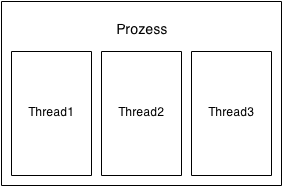
\includegraphics[width=0.3\textwidth]{./data/Threads.png}
	\end{center}
	\vspace{-20pt}
	\caption{Prozess und Threads}
	\vspace{-60pt}
\end{wrapfigure}

\paragraph{Problem}  Die Server-Klasse und Sensor-Klasse befinden sich in einer Endlosschleife, da sie dauerhaft auf eine Eingabe warten. Beim Server sind dies Empfangene Daten und beim Sensor Bewegungssignale. Würden alle Klassen in einem Thread ablaufen, so würde nur eine Klasse gestartet werden und der Anwendungsablauf in dieser bleiben. 
\paragraph{Lösung}  Die beiden oben genannten Klassen, sowie weitere Klassen wie die LED-Steuerung, werden in eigene Threads ausgelagert. Threads sind Unterprozesse im Hauptprozess, die es ermöglichen mehrere Aufgaben in einem Programm gleichzeitig abzuarbeiten. Zwischen den einzelnen Threads kann Datenaustausch statt finden und es ist möglich übergreifende Funktionen aufzurufen. \\
Zur Implementierung wird das Modul 'threading' genutzt. Eine Klasse, die in einem Thread gestartet werden soll, benötigt eine init- und eine run-Methode.
\paragraph{Beispielcode}
Für eine Funktionsdarstellung der Threads mit Python werden drei Klassen angelegt, eine zur Steuerung und zwei, die in einem Thread laufen sollen. \\
Die Klasse 'Testcenter' initialisiert die Klassen als Threads und startet diese.
\begin{lstlisting}[caption=Klasse Testcenter, language=python, frame=single, breaklines=true,columns=fullflexible, commentstyle=\color{gray}\upshape, captionpos=b, numbers = left]
#!/usr/bin/python
# -*- coding: utf-8 -*-
##############################
# Author: Timo Höting                        #
# Mail: mail[at]timohoeting.de            #
##############################
import threading
from TestThread import *
from TestThread1 import *

class TestCenter():
    def newThread(self):
        global testthread
        global testthread1
        testthread = TestThread('thread0', self)
        testthread1 = TestThread1('thread1', self)
        testthread.start()
        testthread1.start()

    def dosth(self):
        print 'dosth'

    def dosth2(self):
        print 'dosth2'

    def dosth3(self):
        testthread1.calledFromMain('-dosth3')

if __name__ == "__main__":
    newThread = TestCenter()
    newThread.newThread()
\end{lstlisting}
Die beiden TestThread-Klassen enthalten beide eine init- und eine run-Methode. Die Klasse Thread1 enthält zusätzlich noch eine Methode die von anderen Klassen ausführbar ist. 
\begin{lstlisting}[caption=Klasse TestThread1, language=python, frame=single, breaklines=true,columns=fullflexible, commentstyle=\color{gray}\upshape, captionpos=b, numbers = left]
#!/usr/bin/python
# -*- coding: utf-8 -*-
##############################
# Author: Timo Höting                        #
# Mail: mail[at]timohoeting.de            #
##############################

import threading
import time
import datetime

class TestThread1(threading.Thread):
    def __init__(self,ms,c):
        threading.Thread.__init__(self)
        global center
        center = c
        global message
        message = ms

    def run(self):
        print message
        center.dosth2()

    def calledFromMain(self, message):
        print  'calledFromMain' + message
\end{lstlisting}
Die init()-Methoden werden bei der Erzeugung des Threads aufgerufen und die run()-Methode wenn er gestartet wird. Danach können die Methoden wie bei normalen Methodenaufrufen benutzt werden. 

\paragraph{Cleanup}
Um die einzelnen Threads korrekt zu beenden sind Methoden zum Aufräumen notwendig. Dies ist vor allem bei Threads wichtig, die sich in einer Endlosschleife befinden oder Server-Anwendung beherbergen. 
\begin{itemize}
	\item \textbf{Webserver:} Im Thread des Twisted-Webservers wird eine Methode implementiert, die den Server korrekt herrunterfährt. Somit wird auch der reservierte Port frei gegeben. 
	\item \textbf{Sensorauswertung:} Die Sensorauswertung befindet sich in einer Endlosschleife, welche beendet werden muss. Die Schleife wird abhängig einer Variable implementiert. In der Cleanup-Methode wird diese Variable auf false gesetzt. 
	\item \textbf{LED-Ansteuerung:} Beim Stoppen der Anwendung müssen alle LEDs ausgeschaltet werden. 
	\item \textbf{Kameraaufnahme:} Da zu Beginn der Aufnahme ein FTP-Verzeichnis gemountet wird, muss dieses am Ende frei gegeben werden. Andernfalls können beim neuen Verbinden Fehler entstehen.
\end{itemize}